\documentclass[main]{subfiles}
\begin{document}

%@@@@@@@@@@@@@@@@@@@@@@@@@@@@@@
% Main Topics: graphs and TU matrices, max-flow min-cut
% Applications of Total Unimodularity - 16.11.2017
% Joe covered Weismantell in this lecture
% author: Vanessa Leite

\section{Applications of Total Unimodularity}

\paragraph{A important reminder:}
Theorem: $A \in \{0, \pm 1\}^{m \times n}$ is TU iff $\forall J \subseteq [n]$
(or $J \subseteq [m]$ because $A^T$ is also TU) $\exists$ partition $J = J_1
\cup J_2$ such that $\sum_{j \in J_1} A_{ij} - \sum_{j \in J_2} A_{ij} \in \{0,
\pm 1\}$ iff $\max \{c^T x \mid Ax \leq b\}$ has an \textbf{integral} optimal
solution for every $b \in \Z^n$, wherever an optimal solution exists, iff $A^T$
is TU.

\paragraph{Definition - Digraph}
Let $V$ be a finite set and $A \subseteq V \times V$. Then $D=(V,A)$ is a
digraph (directed graph).

\paragraph{Definition - Node-arc incidence matrix}
The node-arc incidence matrix of $D=(V,A)$ is the matrix
$M \in \{0, \pm1\}^{\abs{V} \times \abs{A}}$, where $M_{ia} = 
\left\{
  \begin{array}{ll}
    1 & \text{if } (i,j) = a \in A\\
    -1 & \text{if } (j,i) = a \in A \\
    0 & \text{else}
  \end{array}
\right.$

\paragraph{Definition - Node-edge incidence matrix}
The node-edge incidence matrix of an undirected graph $G=(V,E)$ is
$M \in \{0,1\}^{\abs{V} \times \abs{E}}$, where $M_{ve} = 
\left\{
  \begin{array}{ll}
    1 & \text{if } e = (v,w) \in E\\
    0 & \text{else}
  \end{array}
\right.$

\paragraph{Definition -  Edge sets $\delta^+$, $\delta^-$ and $\delta$}
Let $D=(V,A)$ and Let $W \subseteq V$.\\
$\delta^+(W) = \{(i,j) \in A, i \in W, j \notin W \}$, i.e., all the arcs
leaving $W$.\\
$\delta^-(W) = \{(i,j) \in A, i \notin W, j \in W \}$, i.e, all the arcs
entering $W$.\\
Let $G=(V,E)$ and $i \in V$. Then, $\delta(i) = \{(i,j) \in E\}$.

\subparagraph{Example:}
\begin{figure}[!h]
  \centering
    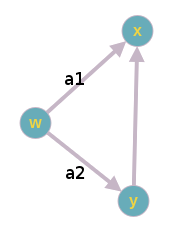
\includegraphics[width=0.2\textwidth]{imgs/graph-definition.png}
\end{figure}

$\delta^+(w) = \{a1,a2\}$.\\
$\delta^-(w) = \emptyset$.\\

\paragraph{Theorem: The following matrices are TU:}
\begin{enumerate}
\item The node-arc incidence matrix of a digraph
\item The node-edge incidence matrix of a bipartite undirected graph
\item An interval matrix, i.e, a $\{0,1\}$ matrix where in each row, the $1$'s
are consecutives.
\end{enumerate}

\subparagraph{Proof:}
\begin{enumerate}
\item Let $M$ be a node-arc incidence matrix of a digraph $D=(V,A)$. Every
column of $M$ has one $1$'s and one $-1$'s. Let $J \subseteq [\abs{V}]$ be a
subset of the rows.
Let $J_1 = J$ and $J_2 = \emptyset$.
Thus, $\sum_{i \in J_1} M_{ij} - \underbrace{\sum_{i \in J_2} M_{ij}}_{=0}
= \sum_{i \in J_1} M_{ij} \in \{0, \pm 1\}^{\abs{A}}$.
\item Let $M$ be a node-edge incidence matrix of a bipartite graph $G=(V,E)$.
Every column of $M$ has two $1$'s. Let $J \subseteq [\abs{V}]$ be a subset
of the rows.
Since $G$ is bipartite, $V = V_1 \cup V_2$. Let $J_1 = J \cap V_1$ and
$J_2 = J \cap V_2$.
Thus, $\sum_{i \in J_1} M_{ij} - \sum_{i \in J_2} M_{ij}
\in \{0, \pm 1\}^{\abs{A}}$.
\item First, observe that for any $J \subseteq \{1, \dots, n\}$, then
$A_{\cdot j}$ still holds the property. Let $J^+$ be the odd columns from $J$
and $J^- = J\setminus J^+$, then for each row $A_{i\cdot}$ we have $\sum_{J^+}
A_{ij} - \sum_{J^-}A_{ij} \in \{0,\pm 1\}$, so, $A$ is TU. 
\end{enumerate}

\paragraph{Maximum stable set problem}

\paragraph{Given $G=(V,E)$, find largest $W \subseteq V$ st no two vertices in
$W$ are adjacent (no edges between them).}

\subparagraph{Example:}
\begin{figure}[!h]
  \centering
    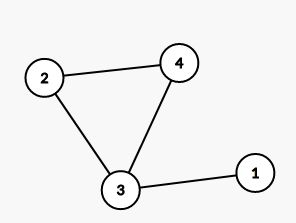
\includegraphics[width=0.3\textwidth]{imgs/graph-stable-set.png}
\end{figure}

Some stable sets are: $\{v_1\}$, $\{v_1, v_2\}$, $\{v_1, v_4\}$, and the
maximum for this graph contains two vertices.

\paragraph{We can model this problem as an ILP}
If we have a cost function $c \in \R^V$, the objective function is written as:
$\sum_{v \in V} x_v c_v$, the constraints are kept the same as in the ILP:
\begin{equation*}
\begin{aligned}
& \max      & & \sum_{v \in V} x_v \\
& \text{st} & & x_v + x_w \leq 1, \; \forall \{v, w\} \in E\\
& & & x_v \in \{0,1\} \; \forall v \in V
\end{aligned}
\end{equation*}

\paragraph{Proposition: If $G$ is bipartite, then the optimal solution to
$\max \{ \sum_{v \in V} x_v \mid x_v + x_w \leq 1, x_v \in [0,1] \}$ is
integral.}

\subparagraph{Proof}
This follows since the constraint matrix is the node-edge incidence matrix of
an undirected bipartite graph.\\
Let $A$ be the node-edge incidence matrix of a bipartite graph $G$. There is a
$1-1$ correspondece between the integral points in $P = \{x \in \R^n_+ \mid
A^T x \leq e\}$ where $e ={1}^{|E|}$ and the stable sets of $G$. Therefore,
optimizing over $P$, which is defined by a TU matrix, yields an integral
solution.

\begin{figure}[!h]
  \label{fig:bipartite-solution}
  \centering
    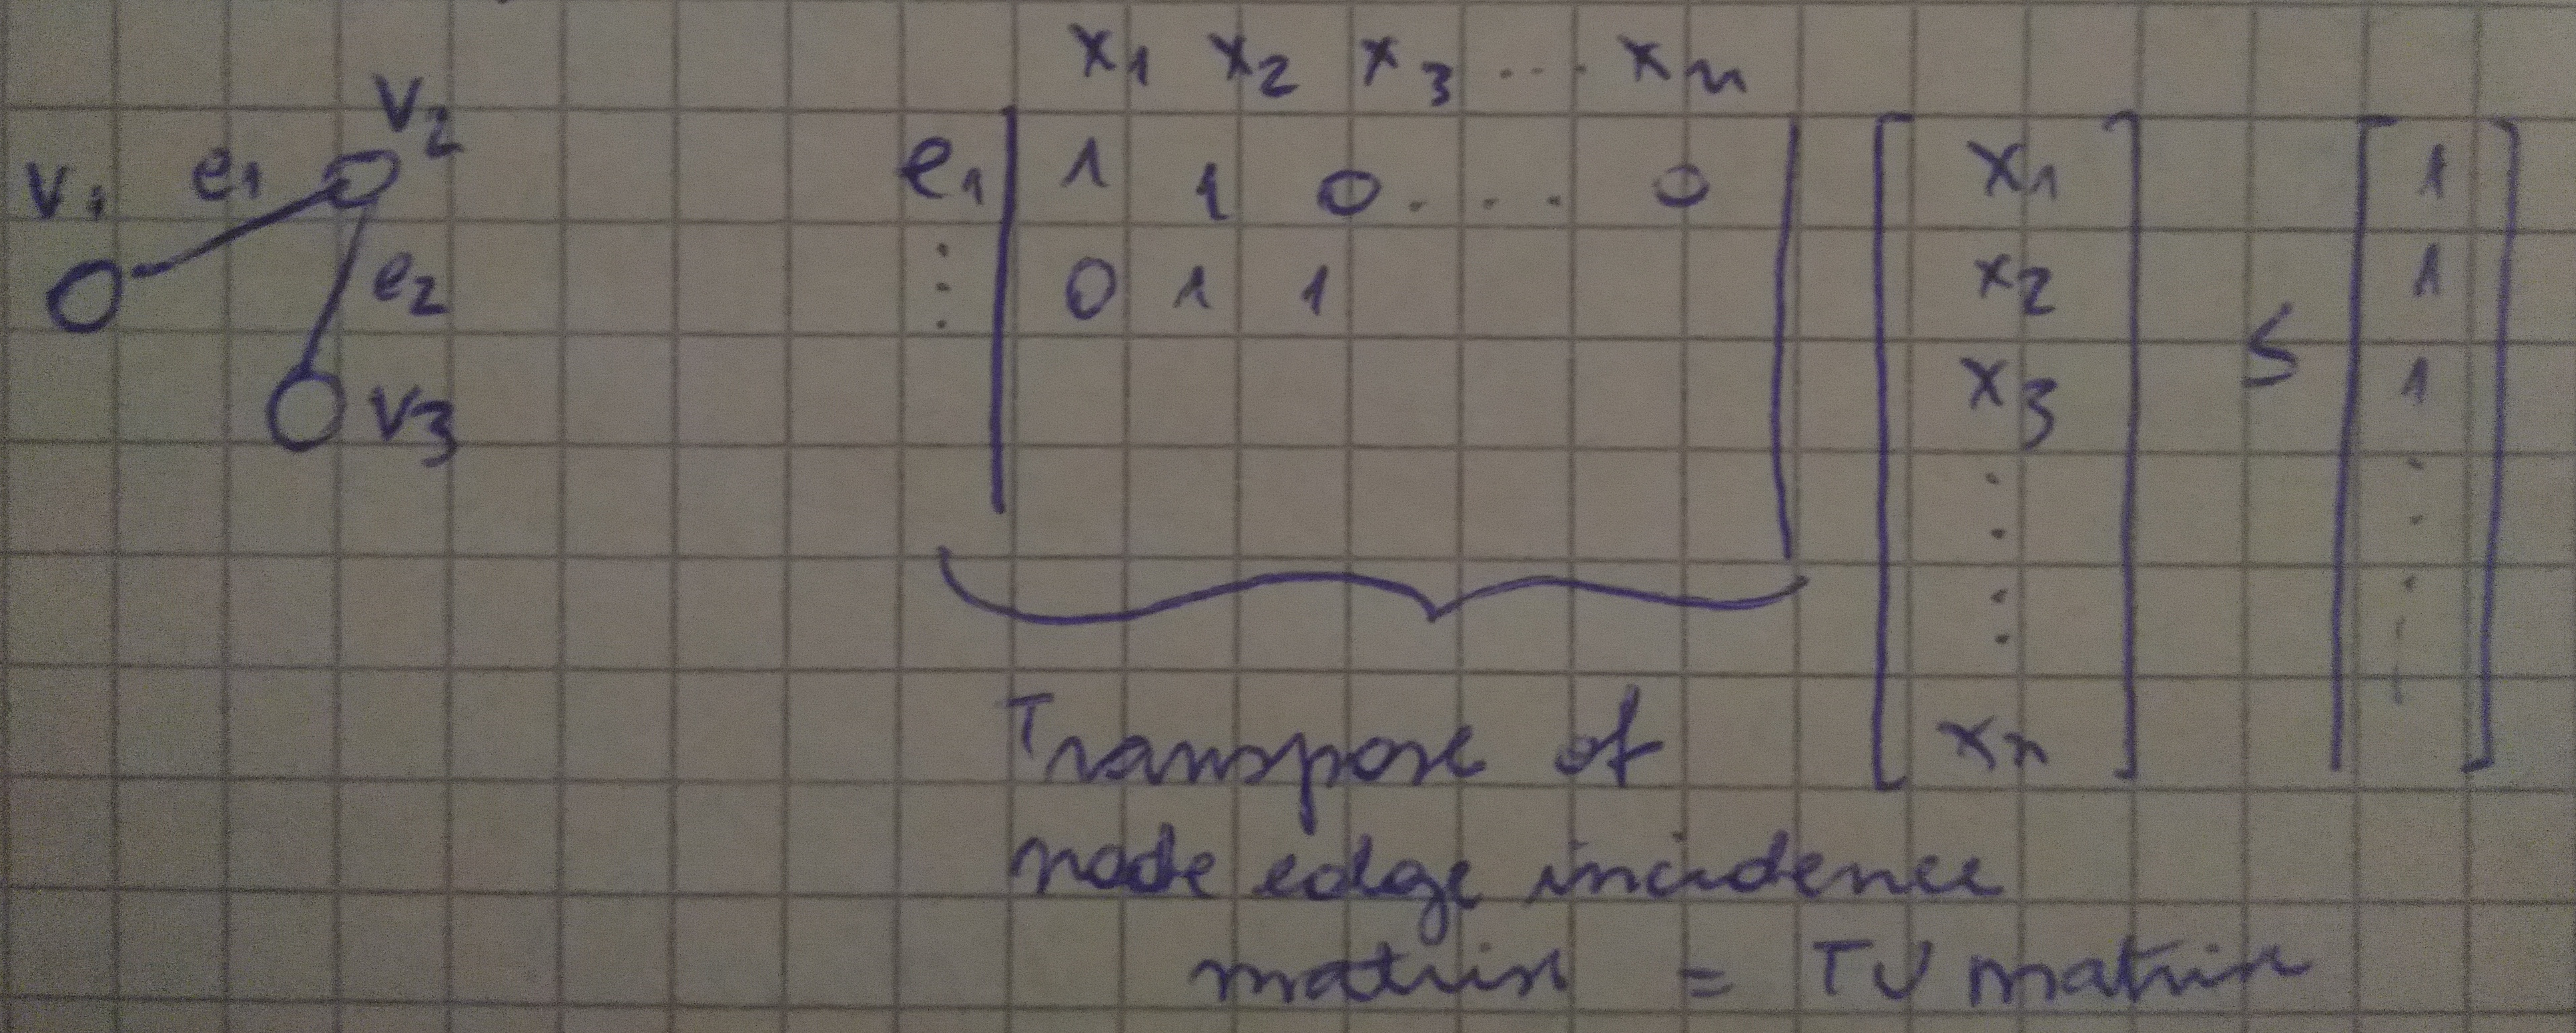
\includegraphics[width=0.5\textwidth]{imgs/bipartite-integral-solution.jpg}
\end{figure}

\paragraph{Definition - (s-t)-flow}
Let $D=(V,A)$ be a digraph. For each $a \in A$, $c_a \in \R_+$ is the \emph{arc
capacity}. Let $s, t \in V$ with $s \neq t$. A function $x: A \mapsto \R$ is an
\emph{(s-t)-flow} if:
\begin{enumerate}
\item flow conservation constraint: $\sum_{a \in \delta^+(v)} x_a = \sum_{a \in
\delta^-(v)} x_a$, $\forall v \in V \setminus \{s, t\}$, i.e., the amount of
flow arriving in an intermediate node must be the same amount that comes out.
\item $0 \leq x_a \leq c_a$ $\forall a \in A$
\end{enumerate}

The value of $x$ is $val(x) = \sum_{a \in \delta^+(s)} x_a - \sum_{a \in
\delta^-(s)} x_a$.

\todo[inline]{check figure on notes}

\paragraph{Theorem: If $c_a \in \Z_+$ for all $a \in A$, then the max value of
an (s-t)-flow can be chosen to be integral.}
\subparagraph{Proof:}
Let $M$ be the node-arc incidence matrix of $D$. Define $b \in \R^{|V|}$ as 
$b_i =
\left\{
  \begin{array}{ll}
  0 \text{ if } i \in V \setminus \{s,t\} \\
  ||c||_1 \text{ if } i \in \{s, t\}
  \end{array}
\right.$

A max (s-t)-flow is the solution to $\max \{ \sum_{e \in \delta^+(s)} x_e - 
\sum_{e \in \delta^-(s)} x_e$ st $-b \leq Mx \leq b$ and $0 \leq x \leq c\}$.
As M is TU, the optimal solution to the problem is integral.

\paragraph{Definition - cut} Let $D=(V,A)$ and $W \subseteq V$. The set
$\delta^+(W)$ is a cut (induced by $W$). An (s-t)-cut satisfies $s \in W$ and
$t \notin W$. Given $c \in \R^{|A|}_+$, the capacity of $\delta^+(W)$ is
$c(\delta^+(W)) = \sum_{a \in \delta^+(W)} c_a$.

\todo[inline]{example on notes}

\paragraph{Lemma: Given $D=(V,A)$ and $s \neq t \in V$, let $x$ be an
(s-t)-flow. For every $W \subseteq V$ st $s \in W$, $t \notin W$, $val(x) =
\sum_{a \in \delta^+(W)} x_a - \sum_{a \in \delta^-(W)} x_a$.}
Intuitively, $val(x)$ is (flow out of $W$) - (flow into $W$).

\subparagraph{Proof}
proof requires some manipulation of definition
\todo[inline]{prove!}

\paragraph{Lemma: Let $x$ be an (s-t)-flow and $\delta^+(W)$ an (s-t)-cut. Then
$val(x) \leq c(\delta^+(W))$, i.e., the amount of the flow is at most the
amount of the cut.}

\subparagraph{Proof:}
Let $x$ be an (s-t)-flow. Let $W \subseteq V$ be such that $s \in W$ and
$t \notin W$. The capacity of the (s-t)-cut induced by $W$ is $c(\delta^+(W))$.
$val(x) = \sum_{a \in \delta^+(W)} x_a - \sum_{a \in \delta^-(W)} x_a$, each
$x$ is bounded by $0$ and $c_a$, then $val(x) \leq \sum_{a \in \delta^+(W)} c_a
- \sum_{a \in \delta^-(W)} 0 = c(\delta^+(W))$.

\paragraph{Theorem: Let $D=(V,A)$, $s \neq t \in V$, $c \in \R^{|A|}_+$. The
max value of an (s-t)-flow is equal to the min capacity of an (s-t)-cut.}

\subparagraph{Proof:}
The max flow can be solved using:
\begin{equation*}
\begin{aligned}
& \max & & z\\
& \text{st} & & x(\delta^-(v)) - x(\delta^+(v)) = 0, \; \forall v \in V
\setminus \{s,t\}\\
& & & x(\delta^-(s)) - x(\delta^+(s)) + z = 0\\
& & & x(\delta^-(t)) - x(\delta^+(t)) - \bar{z} = 0 \\
& & & x_a \leq c_a, \; \forall a \in A \\
& & & x_a \geq 0, \; \forall a \in A
\end{aligned}
\end{equation*}

The dual LP is 
\begin{equation*}
\begin{aligned}
& \min & & \sum_{a \in A} c_a y_a\\
& \text{st} & & y_a + z_v - z_u \geq 0, \; \forall a = (u,v) \in A \\
& & & z_s = 0 \\
& & & z_t = 1 \\
& & & y_a \geq 0, \; \forall a \in A
\end{aligned}
\end{equation*}

let $x^*$ be an optimal solution to LP (max). From previous lemma, it is enough
to find an (s-t)-cut satisfying $val(x^*) = c(\delta^+(W))$. Let $(y^*, z^*)$
be an optimal dual solution and set $w = \{ u \in V \mid z_u^* > 0\}$.\\
If $a=(u,v) \in \delta^+(W)$ then $z_u^* > 0$, $z_v^* \leq 0$.

$y^*_a > 0$. By complementary slackness $x^*_a = c_a$ if $a =(u,v) \in \delta^-
(W)$, then $y^*_a + z_v - z_u > 0$, so, $x^*_a = 0$. Thus, $val(x) = \sum_{a
\in \delta^+(W)} x_a - \sum_{a \in \delta^-(W)} x_a = \sum_{a \in \delta^+(W)}
c_a - \sum_{a \in \delta^-(W)} 0 = c(\delta^+(W))$.

\end{document}
